\chapter{Моделирование}
\section{Инструменты моделирования}
Для нахождения позиции оптимального совмещения волноводов, необходимо смоделировать поле волновода, и вычислить интеграл перекрытия, формула которого приведена в главе \ref{coupling}. Перебирая варианты взаимного расположения полей, необходимо найти максимальное значение этого интеграла.

Перебор всех теоретически возможных вариантов занимает длительное время, поэтому стоит его упростить, предполагая единственный максимум у функции. Для оптимизации поиска экстремумов функции используют методы координатного спуска, градиентного (наискорейшего) спуска и симплекс-метод.\cite{numeric} 

Предполагая, что у искомого распределения значений интеграла перекрытия имеется только один максимум, используем метод градиентного спуска, поскольку в этом случае он позволит достичь результата за меньшее число итераций. \cite{mathews}

Итак, нам нужен инструмент, позволяющий считать интегралы, проводить итерации и строить графики. В работе используется язык программирования Python, имеющий все необходимое. 

Для решения наших задач, к Python подключаются следующие внешние библиотеки:
\begin{itemize}
	\item NumPy - пакет функций для базовых операций с матрицами (создание и итерация по ним)
	\item SciPy - пакет математических функций, используется для интегрирования и содержит реализацию алгоритма градиентного спуска
	\item Mathplotlib - для вывода полученных результатов в виде графиков.
\end{itemize}

Кроме того, для повышения производительности программы, были написаны два вспомогательных модуля, описывающих распределение полей канального и цилиндрического волноводов.

\section{Интерактивная модель}
Для решения основной задачи, то есть поиска точки контакта с максимальным значением коэффициента передачи, было написано отдельное приложение.

\begin{figure}[h!]
	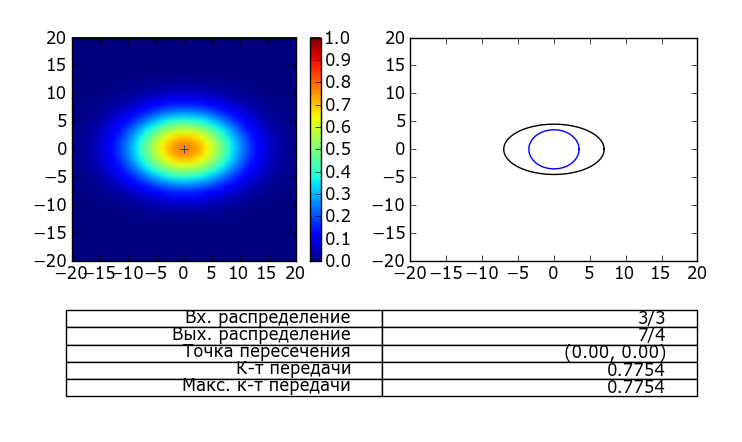
\includegraphics[width=\linewidth]{img/heatmap.png}
	\caption{Общий вид программы}
\end{figure}

В нем показывается вид поля при различных взаимных положениях волноводов. На экране слева показывается поле в выходном волноводе, а справа - схематическое расположение перекрывающихся полей. Ниже показаны числовые значения рассчитываемых параметров. Изначально программа позиционирует волноводы так, чтобы коэффициент передачи был максимален. Кликами по распределению поля можно виртуально изменять положение выходного волновода относительно входного и изображение будет перестраиваться, показывая новое распределение. Таким образом, можно наблюдать что произойдет при отклонении от точки максимального контакта.

\section{Моделирование поперечного смещения}
\label{transverse_section}
Для нахождения точки максимальной эффективности передачи возьмем планарный волновод неподвижным относительно осей координат. Цилиндрический волновод будем перемещать по оси $x$. При смещении волновода максимум распределения также смещается относительно исходного на расстояние $\Delta x$, как показано на рисунке \ref{intersection}. Для исследования коэффициента передачи была написана программа, вычисляющая значения интеграла перекрытия в пределах $x \in [-20, 20]$, мкм.
В моделировании использовались волокна, описанные в \ref{cylinder_field}, которые стыковались к полосковому волноводу, описанному в \ref{strip_field}.

\begin{figure}[h!]
		\includegraphics[width=0.5\linewidth]{img/transversal_courning.png}
		\caption{Зависимость коэффициента передачи из волокна Corning}
\end{figure}
\begin{figure}[h!]
		\includegraphics[width=0.5\linewidth]{img/transversal_fog.png}
		\caption{Зависимость коэффициента передачи из волокна для ВОГ}
		\label{transversal_fog}
\end{figure}

В ходе моделирования, было обнаружены точки наилучшего контакта. Кроме того была обнаружена зависимость коэффициента передачи от радиуса моды. Во втором случае, показанном на рисунке \ref{transversal_fog} максимальное значение составило 64,9\%. Следовательно, возникает задача поиска наилучшего с точки зрения эффективности передачи радиуса моды. Для этого построим график зависимости максимумов передачи для радиусов моды в интервалах от 1мкм до 6мкм включительно.
\begin{figure}[h!]
		\includegraphics[width=0.5\linewidth]{img/var_radius.png}
		\caption{Коэффициент передачи для разных радиусов мод}
\end{figure}

В ходе моделирования получились результаты для радиусов мод многих реальных волокон, а также найден радиус максимального контакта, в при котором происходит почти полная передача энергии - это 2,4~ мкм для данного полоскового волновода. Кроме того видно, что наиболее подходящим из конкретных моделей является волокно, сконструированное специально для ВОГ.

\section{Моделирование продольного смещения}

При продольном смещении необходимо решить задачу нахождения вида пучка на некотором расстоянии от выхода волновода, после чего подставить получившееся распределение в интеграл перекрытия (\ref{coupling}) и определить эффективность передачи.
В моделировании будем использовать планарный волновод, описанный в \ref{strip_field} и цилиндрический с радиусом моды 3~мкм и показателем преломления сердцевины $n$ = 1.47. Длину волны света примем $\lambda$ = 1.55~мкм.

\begin{figure}[h!]
	\includegraphics[width=0.5\linewidth]{img/longitudinal.png}
	\caption{Коэффициент передачи в зависимости от расстояния между волноводами}
	\label{longitudinal}
\end{figure}

По результатам моделирования получился ожидаемый результат. Эффективность передачи падает по мере увеличения расстояния между волноводами. Наибольшее значение как и в предыдущем эксперименте, составило 0.816, поскольку по осям $(x,y)$ мы взяли точку с наивысшим коэффициентом передачи.   